% !TeX root = main.tex
\documentclass[conference]{IEEEtran}
\IEEEoverridecommandlockouts
% The preceding line is only needed to identify funding in the first footnote. If that is unneeded, please comment it out.
\usepackage[utf8]{inputenc} % allow utf-8 input
\usepackage[T1]{fontenc}    % use 8-bit T1 fonts
\usepackage{hyperref}       % hyperlinks
\usepackage{url}            % simple URL typesetting
\usepackage{booktabs}       % professional-quality tables
\usepackage{nicefrac}       % compact symbols for 1/2, etc.
\usepackage{microtype}      % microtypography
\usepackage{lipsum}
\usepackage{fancyhdr}       % header
\usepackage{graphicx}       % graphics
\usepackage{bookmark}
\usepackage{enumitem}

%\usepackage{caption}
\usepackage{svg}
\usepackage{cite}
\usepackage{amsmath,amssymb,amsfonts}
\usepackage{algorithmic}
\usepackage{textcomp}
\usepackage{xcolor}
\usepackage{flushend}
\usepackage{mathtools}
\usepackage[square,sort,comma,numbers]{natbib}
\bibliographystyle{IEEEtranN}
\usepackage{tabularray}
\usepackage{tikz}
\usetikzlibrary{arrows.meta, positioning}
\usepackage{subfig}
\usepackage{listings}
% \usepackage{todonotes}
\usepackage{tabularx}
\usepackage{multirow}
\usepackage{pdfpages}
\usepackage{placeins}
\usepackage{cellspace}
\usepackage{todonotes}
\usepackage{mdframed}
\usepackage{makecell}
\usepackage[most]{tcolorbox}

\newtcolorbox{findingbox}[1][]{
  colback=gray!10!white,
  colframe=gray!50!black,
  #1
}


\setlength\cellspacetoplimit{3.5pt}
\setlength\cellspacebottomlimit{3.5pt}

% \def\BibTeX{{\rm B\kern-.05em{\sc i\kern-.025em b}\kern-.08em
%     T\kern-.1667em\lower.7ex\hbox{E}\kern-.125emX}}
\begin{document}

	\title {Detecting Exception-Related Behavioural Breaking Changes with UnCheckGuard}

    %% \author{\IEEEauthorblockN{Vinayak Sharma\IEEEauthorrefmark{1}, Patrick Lam\IEEEauthorrefmark{2}}
    %% \IEEEauthorblockA{\IEEEauthorrefmark{1}University of Waterloo; \emph{vinayak.sharma1@uwaterloo.ca}}
    %% \IEEEauthorblockA{\IEEEauthorrefmark{2}University of Waterloo; \emph{patrick.lam@uwaterloo.ca}}
    %% }

    \maketitle
    \thispagestyle{plain}
    \pagestyle{plain}

    \begin{abstract}
      The ubiquitous use of third-party libraries in software development has enabled developers to quickly add
      new functionality to their client software. Unfortunately, library usage also carries a cost in
      terms of software maintenance: library upgrades may include breaking changes, in which client expectations
      about library behaviour are no longer met in new library versions. Behavioural breaking
      changes can be particularly insidious, and in their full generality, could require sophisticated program
      analysis techniques to (approximately) detect.

      In this work, we present our UnCheckGuard tool, which detects a class of behavioural breaking changes---those
      related to exceptions thrown by Java libraries. UnCheckGuard analyzes both sides of the library/client
      duet. On the library side, UnCheckGuard creates a list of new exceptions that may be thrown by methods
      in a library's public API, including by its transitive callees. On the client side, UnCheckGuard identifies
      client methods that call library methods with new exceptions. To reduce false positives, UnCheckGuard
      additionally filters out client methods that cannot trigger these new exceptions, using taint analysis. It therefore can be
      used by client developers as a tool to screen library updates for relevant incompatibilities.

      We have evaluated UnCheckGuard on 68 libraries and 98 library-client pairs drawn from the DUETS collection
      and found 8 libraries with newly-added exceptions, as well as 14 callsites to library methods which,
      when upgraded to the latest version, may introduce
      a behavioural breaking change in the client due to a newly added unchecked exception. These findings
      highlight the practical value of UnCheckGuard in identifying exception-related incompatibilities
      introduced by library upgrades.


    \end{abstract}
    
    

    \begin{IEEEkeywords}
        client/library interactions, behavioural breaking changes, exceptions, static analysis
    \end{IEEEkeywords}


    \section{Introduction} \label{sec:introduction}
    % look for citations about library usage
The use of libraries developed by others is ubiquitous in modern
software development~\cite{huang22:_charac_java,wang20:_java}. Libraries enable developers to include
functionality in their own client software without having to
implement it themselves.  However, libraries developed by others are
also updated by others, on schedules that are not controlled by the client developers.

Especially when one is developing software that is exposed to the Internet, one
has a responsibility to incorporate security updates for the
libraries that one is using as a client~\cite{wu23:_under_threat_upstr_vulner_downs}, or else risk vulnerabilities
being exposed in one's software~\cite{haryono22:_autom_ident_librar_vulner_data,zhan21:_atvhun,alfadel23:_empir_python}. The obligation to update libraries is
a form of technical debt that accrues automatically with the passage
of time.

% should we cite our Onward 2020 paper here?
However, upgrading libraries is not painless~\cite{elizalde18:_towar_smoot_librar_migrat,derr17:_keep,dann23:_upcy}: new
versions of libraries may include breaking Application Programming
Interface (API) changes~\cite{dietrich14:_broken}, requiring developers to verify that their own client
code continues working with the new library versions. This is
inconvenient at best and can require nontrivial amounts of software development at worst,
often without the reward of useful new features for the client software---reacting to upgrades
just allows the client software to continue working, in a hopefully less-vulnerable
state.

Compilers and simple static
checkers (including japicmp\footnote{https://github.com/siom79/japicmp} and Revapi\footnote{https://revapi.org/revapi-site/main/index.html} for Java as well as \cite{brito18:_apidif,foo18:_effic_static_check_librar_updat})
can verify the absence of syntactic breaking changes in libraries,
e.g. changes to signatures of public methods, retractions of
formerly-existing methods, or even syntactic changes to library method
implementations. The situation is worse for semantic/behavioural breaking changes:
there do not exist techniques for reliably detecting such changes. Of
course, in its full generality, the problem is undecidable, though
breaking change detection could be estimated using static and dynamic program analysis
techniques.

In this work, we contribute a novel way to detect one type of behavioural breaking
change in a library. Our work enables client developers to inspect relevant changes
to the set of exceptions that may be thrown by a Java library, particularly
by the APIs that are actually used by specific client code. A new exception thrown by a library
constitutes a breaking change; uncaught exceptions can cause the client to crash or
to exhibit unexpected behaviour.

Although developers tend to ignore even checked
exceptions~\cite{nakshatri16:_analy_java}, we contend that incrementally informing
developers only about relevant newly-added exceptions is more likely to result in developer action, consistent with the
design principles of Google's Tricorder tool~\cite{sadowski15:_tricor}.
Thus, we leverage taint analysis
to reduce the number of irrelevant reports that we report to client developers.
We aim to show only changed library APIs that may realistically throw new exceptions
in updated versions of client code, minimizing the number of false positives~\cite{pashchenko20:_vuln4,pashchenko18:_vulner}.
We hope that our reports enable client developers to better understand how new exceptions affect their own code.

We explore the following research questions:

\noindent
{\bf RQ1.} Do library clients call methods with new added exceptions, and is it possible for the clients to trigger these exceptions? Furthermore, is it possible to write client-focussed test cases that trigger the exceptions?

\noindent
{\bf RQ2.} For library changes that introduce triggerable new unchecked exceptions, under what circumstances do such exceptions occur (i.e. major/minor/patch versions)?


In our corpus of 302 distinct libraries, we found 120 libraries with newly-added exceptions, including exceptions that are added in non-major releases.
We then investigated 352 client-library pairs to explore the prevalence of potentially breaking behavioural changes.
We found that new potentially client-relevant unchecked exceptions occured in 120 of the 302 libraries, and that clients called methods reaching these exceptions at 1708 client callsites.
This shows that client applications do in fact call library methods that throw these new exceptions.
Furthermore, we demonstrated that it is possible to trigger these exceptions by writing test cases using methods from the client.

The contributions of this work are as follows:

\begin{itemize}[noitemsep]
\item We implement the \textit{UnCheckGuard} static analysis tool, which traverses bytecode to find newly-added exceptions and filters them using taint analysis, to report relevant newly added unchecked exceptions.
\item We conduct an empirical study of libraries to detect potential behavioural breaking changes in libraries caused by newly added unchecked exceptions.
\item We evaluate 352 client-library pairs from the DUETS dataset~\cite{durieux21:_duets} using \textit{UnCheckGuard}, identifying 1708 call sites where libraries' newly added unchecked exceptions could cause behavioural breaking changes in clients, and write test cases showing that the exceptions can be triggered from client code.
\end{itemize}

\noindent \textbf{Data Availability Statement.}

\indent We have made our tool and dataset available at \url{https://doi.org/10.5281/zenodo.16788650}


%RQ1: Do libraries have breaking changes in the form of added exceptions?
%RQ2: Do clients call the methods which have these breaking changes, and can we trigger the new exceptions?

%true, [RQ1] I think even logically it would make sense to showcase that libraries do add new unchecked exceptions (UE). We can even do something about the version in which they are adding the UE (do they introduce the UE in major version or minor version or patch version). [RQ2] Then we can follow it up with how often do clients call such method which have a newly added UE and can we trigger those UE (the taint analysis part can be defended along with it). 

% https://hasel.auckland.ac.nz/2023/11/12/understanding-breaking-changes-in-the-wild/


    \section{Motivating Example} \label{sec:motivating}
    We continue with a motivating example drawn from the DUETS collection~\cite{durieux21:_duets}
of client/library pairs. 
In our example,
a revision of the \texttt{httpcore} library\footnote{https://hc.apache.org/index.html} adds a check for an
error condition.  If the condition evaluates to true, the library method will
explicitly throw an \texttt{IllegalArgumentException}. The client, \texttt{HttpAsyncClientUtils}\footnote{\url{github.com/a63881763/HttpAsyncClientUtils}},
calls the relevant part of the library, and thus may be affected by the new exception.

In the DUETS suite, our client, \texttt{HttpAsyncClientUtils}, declares a dependency on
version 4.4.6 of the \texttt{httpcore} library. Between the release of DUETS and today, the \texttt{httpcore} developers
have released a number of new versions, and at the time of writing, the latest version of \texttt{httpcore}
is 4.4.16\footnote{While \texttt{httpcore} 5.2.4 is in fact the latest version of this library, the library developers have released \texttt{httpcore5} as a distinct Maven component from \texttt{httpcore4}, and labelled \texttt{httpcore}(4) as end-of-life.}.

\paragraph{Library} All constructors for the \texttt{org.apache.http.HttpHost} class transitively call
the static method \texttt{Args.containsNoBlanks()}. Between version 4.4.6 and version 4.4.16, the \texttt{httpcore}
developers added the following lines of code to \texttt{containsNoBlanks()}:
\begin{lstlisting}[language=Java]
  if (argument.length() == 0) {
    throw new IllegalArgumentException
      (name + `` may not be empty'');
  }
\end{lstlisting}
Specifically, all \texttt{HttpHost} constructors take a \texttt{hostname} parameter and call \texttt{containsNoBlanks()}
with that parameter (to check that it contains no blanks). It is therefore possible to trigger this newly-thrown
exception in a client by attempting to instantiate a new \texttt{HttpHost} object and passing it an empty
\texttt{hostname}.

Our UnCheckGuard tool analyzes the change in \texttt{httpcore} and finds that, in
version 4.4.16, all of the \texttt{HttpHost} constructors may now throw an
\texttt{IllegalArgumentException} via the \texttt{containsNoBlanks()} method.
This exception was not thrown in 4.4.6.

To detect this change, UnCheckGuard processes JAR files for both \texttt{httpcore-4.4.6} and \texttt{httpcore-4.4.16}. It uses SootUp~\cite{Karakaya24:_sootup} to construct a call graph using Class Hierarchy Analysis (CHA) starting from the public \texttt{<init>(String, int)}\footnote{Specifically, constructor \texttt{<init>(String, int)} returning a \texttt{void} on class \texttt{org.apache.http.HttpHost}} constructor on \texttt{HttpHost} and identifies the set of all transitively reachable methods. UnCheckGuard then collects all unchecked exceptions thrown within this set of reachable methods, for both library versions.

\paragraph{Client} 
A newly-added exception is only relevant to a particular client if that client may
potentially trigger that exception.  It turns out that
our \texttt{HttpAsyncClientUtils} client has reachable code from its public \texttt{createAsyncClient(boolean)}\footnote{Fully-qualified: method \texttt{createAsyncClient(boolean)} returning a \texttt{CloseableHttpAsyncClient} on class \texttt{Util.HttpClientUtil.HttpAsyncClient}.} method
that creates an \texttt{HttpHost} with an empty \texttt{host}. This
method takes a \texttt{proxy}
parameter and contains the following code:
\begin{lstlisting}[language=Java,basicstyle=\scriptsize\ttfamily]
 if (proxy) {
  return HttpAsyncClients.custom()
   .setConnectionManager(conMgr)
   .setDefaultCredentialsProvider(credentialsProvider)
   .setDefaultAuthSchemeRegistry(authSchemeRegistry)
   .setProxy(new HttpHost(host, port))
   .setDefaultCookieStore(new BasicCookieStore())
   .setDefaultRequestConfig(requestConfig).build();
 } else {
   // ...
\end{lstlisting}
where \texttt{host} is a private field initialized to the empty string.
Thus, calling \texttt{createAsyncClient(true)} triggers an exception when executed with
\texttt{httpcore} version 4.4.16 but not with 4.4.6.

To detect that our \texttt{HttpAsyncClientUtils} client calls a method from \texttt{httpcore-4.4.6} which, upon upgrading to \texttt{httpcore-4.4.16}, may throw a new unchecked exception, UnCheckGuard begins by identifying all external library methods invoked anywhere in the client. It then analyzes both the current and the latest versions of the library.

Using this analysis, it determines whether any newly introduced unchecked exceptions are reachable from the client's code. Here, reachability means that the client can trigger the exception in the library on some execution of the program, using values it passes to the library as parameters.

To check if the client-supplied values can reach the exception-throwing site, we use taint analysis as implemented using FlowDroid~\cite{Arzt14:_flowdroid}. Taint analysis is essential in this scenario because the existence of a path from the client callsite to an exception-throwing statement is not sufficient to conclude that the exception is actually triggerable by the client. We found that many such paths may exist in a library, but the control-flow conditions leading to the exception might depend entirely on internal library values, rather than on client-supplied inputs; the client cannot trigger the exception. Therefore, taint analysis becomes necessary to distinguish actual behavioural breaking changes from false positives.

Specifically, we use taint analysis to track whether any client-supplied method parameters (source) can propagate to the exception object's constructor (sink). If taint analysis determines that no client-supplied input flows into the exception-triggering logic, then we can conclude that the newly added exception will not cause a behavioural breaking change, and we do not report that exception.
%For exceptions that we report, we know that a path exists in the interprocedural control-flow graph (which one can compute with CHA) from the client method to the statement throwing the exception in the library.

In version 4.4.6, UnCheckGuard finds two sites throwing \texttt{IllegalArgumentException}, while in 4.4.16, it detects three—each of which the client can potentially trigger using the values it chooses to pass to the library as parameters.

Based on FlowDroid's confirmation of the reachability of the new exception's constructor, we report that the library-client pair \texttt{HttpAsyncClientUtils} and \texttt{httpcore} exhibits a behavioural breaking change.

Given this report, it is straightforward to write a test case that calls the client's \texttt{createAsyncClient()} method
and triggers the exception after an upgrade:
\begin{lstlisting}[language=Java,basicstyle=\scriptsize\ttfamily]
@Test
void testCreateAsyncClientThrowsExceptionForEmptyProxyHost() {
  HttpAsyncClient client = new HttpAsyncClient();

  IllegalArgumentException exception =
    assertThrows(IllegalArgumentException.class, () -> {
        client.createAsyncClient(true);
    });

    assertTrue(exception.getMessage()
    .contains("may not be empty"),
      "Expected exception due to empty hostname "+
      "after upgrading to httpcore-4.4.16");
}
\end{lstlisting}


    %\section{Background}\label{sec:background}
    %\input{background}


    \section{Data Collection}\label{sec:data-collection}
    This section describes the systematic approach we used to construct the dataset for our study on behavioral incompatibilities caused by newly added unchecked exceptions in upgraded Java libraries. 

Broadly, we require three key components: Java-based clients that depend on third-party libraries, the current versions of the libraries used by these clients, and the latest available versions of those same libraries. For each client-library pair, we also need to extract the set of unchecked exceptions thrown by the library methods actually used by the client.

To obtain this information, our methodology involves several key steps: identifying suitable Java clients, extracting their library dependencies, resolving both the current and latest versions of the libraries, analyzing exception behavior in both versions, and recording all methods that introduce newly added unchecked exceptions. 

Each step is essential for enabling our tool, UnCheckGuard, to pinpoint client call sites that may be affected by behavioral breaking changes.

\subsection{Collecting Clients}

To begin our analysis, we first collected suitable client projects. We used the DUETS dataset~\cite{durieux21:_duets}, which provides a curated list of Java-based clients hosted on GitHub, each with at least five stars. We attempted to download each client repository and discarded any client that failed to download.

Next, we checked whether the project included a \texttt{pom.xml} file, which indicates that it is a Maven-based project. This step was essential, as our analysis depends on running Maven commands. We compiled each client to produce a JAR file and kept only those clients that compiled successfully for further analysis.

\subsection{Library Version Resolution}

A core component of our tool relies on analyzing both the version of the library currently used by the client and the latest available version. To collect the current version, we run the Maven command \texttt{mvn dependency:copy-dependencies}, which downloads all the dependencies declared in the client's build configuration.

To obtain the latest versions of these dependencies, we run the following Maven command:
\begin{lstlisting}[language=bash, breaklines=true, basicstyle=\ttfamily\small]
mvn org.codehaus.mojo:versions-maven-plugin:2.18.0:use-latest-versions
\end{lstlisting}
This command updates the \texttt{pom.xml} file with the most recent versions of all declared dependencies. We then re-run \texttt{mvn dependency:copy-dependencies} to download the updated set of libraries.

By following this process, we obtain both the original and the upgraded versions of each library used by the client, enabling us to perform a comparative analysis of behavioral changes across versions.

\subsection{Method and Exception Extraction}

We analyze the JAR file of the client application using SootUp to extract all external method invocations performed by the client. Based on the recorded method calls, we analyze both the currently used version of the library and its latest available version.

To support this comparison, we also extract the list of methods present in the current version of the library. This allows us to match each external method call made by the client to its corresponding definition in the library. Using this information, we generate a JSON file that contains only the subset of library methods actually used by the client. This filtered list enables more focused and efficient analysis in subsequent steps.

\subsection{Comparing Library Versions}

Our tool detects newly added unchecked exceptions using static analysis and verifies them using taint analysis. After collecting the unchecked exceptions from both the old and the latest versions of the library, we compare the sets of exceptions associated with each method. We remove any duplicate exceptions that appear in both versions. If a method in the latest version throws an exception that was not present in the older version, we tag that method as having a newly added unchecked exception.

Using the previously generated mapping between client call sites and library methods, we create a JSON file that lists each client method along with the corresponding external method call that triggers a newly added unchecked exception. This output enables our tool to highlight call sites in the client application that may exhibit behavioral breaking changes, helping developers assess the impact of upgrading their dependencies.



    \section{Methodology}\label{sec:methodology}
    The previous section, Section~\ref{sec:data-collection}, described how we collected the clients and libraries, as well as the necessary information to perform our analysis.
In this section, we describe our methodology for detecting and verifying newly added unchecked exceptions in a library when it is updated from an older version to a newer one. Our focus is on identifying the impact of such changes on client code. Specifically, we analyze client programs to detect usage of library methods that were updated to throw previously non-existent unchecked exceptions. Java distinguishes between checked exceptions, which appear as part of method signatures, and unchecked exceptions, which do not. Unchecked exceptions may therefore introduce a class of breaking changes that method signature-based syntactic approaches for Java cannot detect.

After carrying out the data collection steps in Section~\ref{sec:data-collection} and extracting all external library methods invoked by the client, we next analyze their implementations, in both the current version and the latest version. This allows us to compare their behaviour across versions. If we find, through our analysis, that a method now throws a newly added unchecked exception in the latest version, and that the exception can be triggered from the client code, we flag a potential behavioural breaking change. To verify whether this change is in fact breaking, we currently manually write test cases to verify that the client may be affected by the newly introduced exception. We found that this was easy to do given the information that UnCheckGuard reports.

\subsection{Analysis Setup}

\begin{figure*}[hbt!]
    \centering
    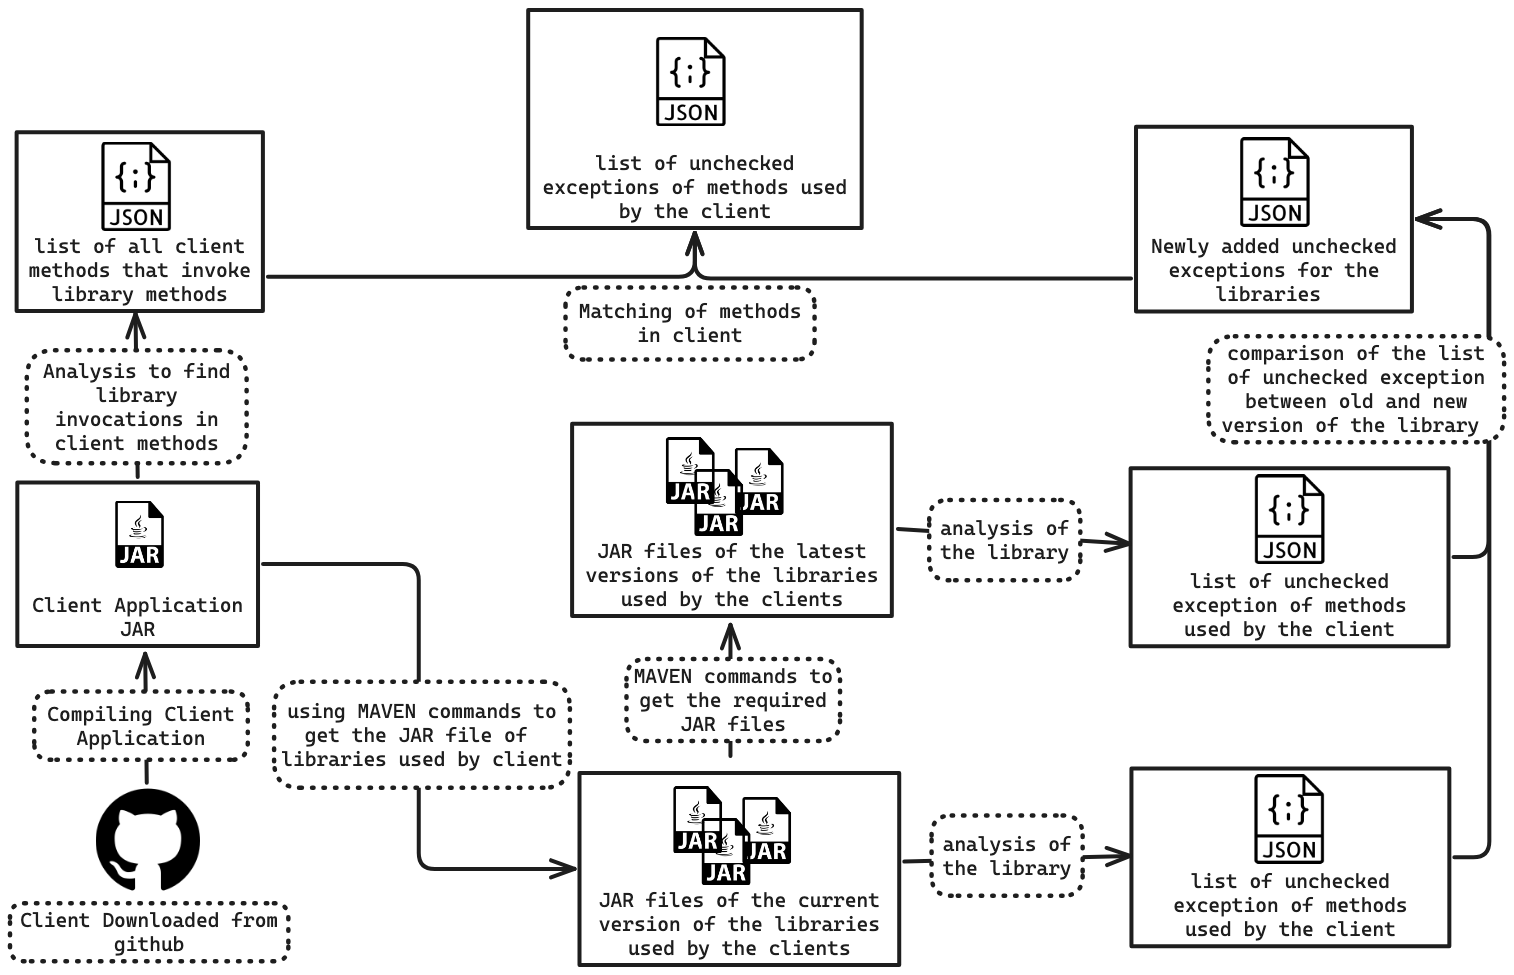
\includegraphics[height=260pt]{diagram/finalPipeline.png}
    \caption{Pipeline of UnCheckGuard for detecting behavioural breaking changes due to newly added unchecked exceptions.}
    \label{fig:jsonjava}
\end{figure*}

The analysis setup is divided into two main phases: client selection and knowledge extraction for analysis. An overview of the full pipeline is shown in Figure~\ref{fig:jsonjava}.

As described in Section~\ref{sec:data-collection}, we begin by selecting Java-based clients from the DUETS dataset~\cite{durieux21:_duets}. We retain only those clients that are Maven-compatible and successfully compile to a JAR file, ensuring compatibility with our analysis tooling.

After selecting the valid clients and compiling them into JAR files, we proceed to extract relevant method-level knowledge from both the client and the current version of the libraries it depends on.

We use SootUp~\cite{Karakaya24:_sootup} to analyze the client JAR and identify all external method invocations. UnCheckGuard performs this analysis by traversing the Jimple intermediate representation of each client method and checking whether any statement contains an \texttt{InvokeExpr}, which represents a method invocation. For each invocation, we retrieve the declaring class type\todo{per our discussion about inheritance, it is possible, though unlikely, that the client invokes on a standard library method and the actual target is in the library.} of the target method. We then check whether this class type is part of the client’s SootUp view---essentially, whether it was declared in the client JAR file plus Java standard library. If the class type is not found in the view, we mark the method as external. This process allows us to filter out internal method calls and focus only on invocations to external library methods.

In parallel, we analyze the current (i.e., pre-upgrade) version of each library used by the client. Using SootUp, we extract all method signatures defined in the library JAR. We then match each external method call made by the client to the corresponding method in the library by comparing their fully qualified method signatures\todo{this doesn't completely work, it's not C, there is dynamic dispatch; for instance, client may have a call to List.add() and library defines LinkedList.add and ArrayList.add() - pending}. This one-to-one mapping enables us to identify exactly which library methods are invoked by which client methods.

At the end of this stage, we produce a structured mapping between client methods and the external library methods they invoke. This mapping serves as a foundation for later stages in our analysis, where we detect behavioural changes in upgraded library versions and trace their potential impact on client call sites.

\subsection{Finding Newly Added Unchecked Exceptions}

Our primary goal is to detect whether upgrading a library introduces new unchecked exceptions that could affect client behaviour. To achieve this, we divide the process into two stages: first, identifying newly added unchecked exceptions using a call graph; and second, verifying their reachability from client input using a taint analysis.

\subsubsection{Exception Discovery with RTA}

To detect newly added unchecked exceptions in the upgraded library, we first construct a call graph using Rapid Type Analysis~\cite{bacon96:_fast_static_analy_c_virtual_funct_calls} (RTA) via SootUp~\cite{Karakaya24:_sootup}. We use RTA instead of Class Hierarchy Analysis (CHA) because RTA provides a more precise approximation of runtime behaviour in the context of a particular client/library pair. CHA, working on the class hierarchy, includes all methods defined in subclasses and interface implementations regardless of whether they are actually invoked. RTA instead considers only those types that are instantiated in the program (client plus libraries), resulting in a more accurate call graph.

By definition, CHA reports the most conservative soundy~\cite{livshits15:_in} answer possible, absent reflection and other dynamic features. Thus, it tends to over-approximate and report unreachable method calls. For example, in one case, CHA identified a path from the public \texttt{getString(String)}\footnote{Fully-qualified name: method \texttt{getString(String)} returning a \texttt{String} on class \texttt{com.alibaba.fastjson.JSONObject}} method, reporting an exception thrown in the \texttt{JSONObject} constructor as reachable. However, manual inspection revealed that this path was spurious—the method \texttt{getString} never reaches the constructor in question because, in the specific program under analysis, no code instantiates a \texttt{JSONObject}. RTA excludes such paths because it considers only types that are actually instantiated, whereas CHA includes all potential subtype relationships, regardless of runtime feasibility.
% we should probably make this whole discussion more concise when we have space limitations

After building the RTA-based call graph, we traverse the entire callgraph and collect all exceptions that are subclasses of \texttt{java.lang.RuntimeException} or \texttt{java.lang.Error}. Per the definition of the Java programming language, such exceptions represent the complete set of unchecked exceptions that the client might be newly exposed to due to the library upgrade.

\subsubsection{Exception Verification with Taint Analysis}

Once we collect the list of unchecked exceptions, we need to determine which of them can actually be triggered by client inputs. This is necessary because many exceptions that show up during call graph analysis are not reachable in practice—they rely on internal values rather than any parameters the client supplies. To filter out such cases, we use FlowDroid~\cite{Arzt14:_flowdroid}, a static taint analysis framework.

Consider the following case drawn from our corpus. The client \texttt{4ntoine/ServiceDiscovery-java}\footnote{\url{https://github.com/4ntoine/ServiceDiscovery-java}} uses the method \texttt{copyFromUtf8(String)} from the library \texttt{protobuf-java-2.6.1}. When this library is upgraded to \texttt{protobuf-java-4.30.1}, the method's implementation adds a new unchecked exception—an \texttt{IllegalArgumentException}. Our tool initially flags this as a behavioural breaking change because the exception is present in the upgraded version and not in the previous one, and because there is a interproceddural control-flow path from the client method to the callsite where the exception is thrown.

However, a closer inspection shows that this exception cannot be triggered by any value passed from the client. The method that throws the exception looks like this:

\begin{lstlisting}[language=Java,breaklines=true,basicstyle=\scriptsize\ttfamily]
static CodedInputStream newInstance(
    final byte[] buf, final int off, final int len, final boolean bufferIsImmutable) {
  ArrayDecoder result = new ArrayDecoder(buf, off, len, bufferIsImmutable);
  try {
    result.pushLimit(len);
  } catch (InvalidProtocolBufferException ex) {
    // The only reason pushLimit() might throw an exception here is if len
    // is negative. Normally pushLimit()'s parameter comes directly off the
    // wire, so it's important to catch exceptions in case of corrupt or
    // malicious data. However, in this case, we expect that len is not a
    // user-supplied value, so we can assume that it being negative indicates
    // a programming error. Therefore, throwing an unchecked exception is
    // appropriate.
    throw new IllegalArgumentException(ex);
  }
  return result;
}
\end{lstlisting}

In the comment written by the library developer, the developer states that this exception cannot be thrown by this non-public method, essentially because \texttt{len} cannot be directly supplied by a client. Our taint analysis confirms that no source for len flows into the sink (exception)\todo{What are the possible sources?}. This shows the importance of having taint analysis to verify whether the exception can actually cause a behavioural breaking change in the client.

To enable taint analysis, we automatically generate a \textit{driver stub} for each library method used by the client. We generate this stub because, to our knowledge, FlowDroid does not allow marking method parameters directly as sources. Instead, we wrap each parameter in a synthetic method whose return value is marked as a source. This approach allows us to simulate tainted inputs and track their flow through the library method. Stub generation, implemented using SootUp, handles a variety of cases, including:
\begin{itemize}
  \item Constructor methods (\texttt{<init>} using \texttt{new ClassName(...)})
  \item Static and instance methods
  \item Void and non-void return types
  \item Primitive parameters (e.g., \texttt{int} $\rightarrow$ \texttt{0})
  \item Object parameters (defaulted to \texttt{null})
  \item Nested classes (converting \texttt{\$} to \texttt{.})
  \item Multiple parameters (sources named \texttt{SourceN()}, where $N$ is the parameter index)
  \item Overloaded methods (only one version retained)
\end{itemize}

An example of a driver stub follows.
\begin{lstlisting}[language=Java,breaklines=true,breakatwhitespace=false,basicstyle=\scriptsize\ttfamily]
public class DriverStub {

    public static java.lang.String source0() {
        return null;
    }

    public static void run() {
        int result = new com.alibaba.fastjson.JSONObject().getIntValue(source0());
    }
}
\end{lstlisting}

In the above example of the driver stub, we generate a stub for the public \texttt{getIntValue(String)}\footnote{Fully-qualified name: method \texttt{getIntValue(String)} returning a \texttt{int} on class \texttt{com.alibaba.fastjson.JSONObject}} method, which belongs to the library \texttt{fastjson-1.2.58}. It has a method parameter of type \texttt{java.lang.String}, which we declare as a method named \texttt{source0} in the driver stub. We declare the method \texttt{source0} to be a source, as FlowDroid marks its return value as a source. We generate the way \texttt{getIntValue} is called based on the type of method it is, and obtain the properties of the method using SootUp.

We treat each exception discovered in the RTA phase as a \textit{taint sink}. For this analysis, we intentionally construct the call graph using Class Hierarchy Analysis (CHA). Although CHA is less precise than RTA, it offers conservative coverage, reducing the risk of missing true positive flows due to aggressive pruning.

Consider the following method from the \texttt{beam-sdks-java-core} library:

\begin{lstlisting}[language=Java,breaklines=true,breakatwhitespace=false,basicstyle=\scriptsize\ttfamily]
public static void applicableTo(PCollection<?> input) {
 WindowingStrategy<?, ?> ws = input.getWindowingStrategy();
 if (ws.getWindowFn() instanceof GlobalWindows
     && ws.getTrigger() instanceof DefaultTrigger
     && input.isBounded() != IsBounded.BOUNDED) {
  throw new IllegalStateException("...");
 }
}
\end{lstlisting}

\begin{figure}[t]
\centering
\scalebox{0.75}{
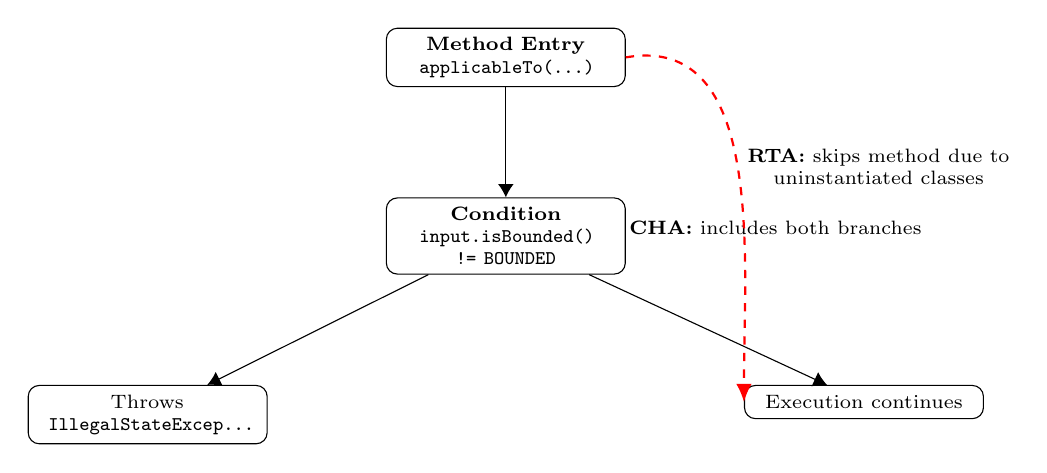
\begin{tikzpicture}[
  node distance=1.4cm and 1.5cm,
  box/.style={rectangle, draw, rounded corners, minimum height=1.2em, text width=2.8cm, align=center, font=\scriptsize},
  every edge/.style={draw, -{Latex[width=2mm]}},
  rededge/.style={draw=red, thick, dashed, -{Latex[width=2mm]}}
  ]

% Nodes
\node[box] (start) {\textbf{Method Entry}\\ \texttt{applicableTo(...)}};
\node[box, below=of start] (cond) {\textbf{Condition}\\ \texttt{input.isBounded() != BOUNDED}};
\node[box, below left=of cond] (exc) {Throws \\ \texttt{IllegalStateExcep...}};
\node[box, below right=of cond] (noexc) {Execution continues};

% Edges
\path (start) edge (cond);
\path (cond) edge (exc);
\path (cond) edge (noexc);

% Labels
\node[align=left, font=\scriptsize] at ([xshift=1.9cm,yshift=0.1cm]cond.east) {\textbf{CHA:} includes both branches};
\draw[rededge] (start.east) to[out=10,in=90] node[right, align=center, font=\scriptsize] {\textbf{RTA:} skips method due to\\ uninstantiated classes} (noexc.west);

\end{tikzpicture}
}
\vspace{-1ex}
\caption{CHA vs. RTA: RTA only reaches the \texttt{IllegalStateException} if types like \texttt{GlobalWindows} or \texttt{DefaultTrigger} are instantiated in the analyzed code.}
\label{fig:rta-vs-cha}
\vspace{-2ex}
\end{figure}


In this example, the parameter \texttt{input} is the taint source, and the \texttt{IllegalStateException} is the sink. The public \texttt{applicableTo(PCollection)}\footnote{Fully-qualified name: method \texttt{applicableTo(PCollection)} returning a \texttt{void} on class \texttt{org.apache.beam.sdk.transforms.GroupByKe}} method is used by the \texttt{0xdecaf/beam-enrichment-patterns}\footnote{\url{github.com/0xdecaf/beam-enrichment-patterns}} client.

RTA excludes types that are never instantiated in the analyzed program. It is more precise and reaches the exception only if actual runtime types lead to the throw statement. In contrast, CHA is more conservative. In this case, RTA reaches the \texttt{IllegalStateException} only if classes such as \texttt{GlobalWindows} or \texttt{DefaultTrigger} are instantiated in the analyzed codebase. CHA, on the other hand, includes all possible overrides regardless of whether those types are instantiated. As a result, even if the actual runtime types are unused, CHA still explores all feasible paths and reaches the IllegalStateException. As shown in Figure~\ref{fig:rta-vs-cha}, this broader approximation allows taint analysis to identify exception flows that RTA would miss due to its stricter instantiation-based filtering.\todo{I still don't believe this: if GlobalWindows or DefaultTrigger are never invoked, why does it matter?}

% RTA excludes types that are never instantiated in the analyzed program. As a result, if no code in the client or the library instantiates a \texttt{PCollection}, the method \texttt{applicableTo(PCollection)} may not appear in the RTA-generated call graph at all. This exclusion causes the exception thrown in that method to be missed. In contrast, CHA includes all types from the class hierarchy regardless of instantiation, so the method is included in the call graph along with the conditional path to the exception. As shown in Figure~\ref{fig:rta-vs-cha}, this broader approximation allows the taint analysis to identify exception flows that RTA would miss due to its stricter instantiation-based filtering.

This trade-off justifies the use of CHA in the filtering phase: although it may over-approximate in some cases, it ensures that no critical exception flows are missed.

After collecting the list of unchecked exceptions for each method in both the old and latest versions of the library, we perform a comparison to identify newly introduced exceptions. If a method exists in the old version but is missing from the latest version, we exclude it from our analysis, as its removal may indicate a method signature–based breaking change, which is handled by existing tools and lies outside the scope of our detection.

For methods that appear in both versions, we compare the sets of unchecked exceptions that they throw. We perform this comparison using both the exception type (e.g., \texttt{java.lang.IllegalArgumentException}) and the fully qualified signature of the method in which the exception occurs. If, after removing all exceptions common to both versions, the method in the latest version still contains any additional unchecked exceptions, we classify it as a method with a newly added unchecked exception. Otherwise, we discard it from further consideration; our technique cannot find new exception-related behavioural breaking changes for this library method.

\subsection{Filtering Untriggerable Unchecked Exceptions}

Based on the information collected about newly added unchecked exceptions, we use the previously generated client-to-library method mapping to determine which client methods invoke a library method that now throws a new unchecked exception. This step allows us to identify specific client call sites that may be affected by behavioural breaking changes introduced in the upgraded library version.

To validate the practical impact of these changes, we manually write test cases to assess whether the client can actually trigger the exception. Each test case is constructed starting from the client call site identified in the mapping. We then examine the method that was flagged as containing a newly added unchecked exception. This information is available in the JSON output produced by our tool, which includes the exception type and the method signature in which it occurs.

The JSON output helps us locate the exact exception-throwing line in the library, which enables a detailed inspection of how the exception is triggered. We first test the exception by directly calling the relevant library method with crafted parameters. If this call triggers the exception, we proceed to construct a full test case that invokes the client method, propagating the same parameter values.

In some scenarios, we are unable to trigger the exception through the client due to certain code structures:
\begin{itemize}
  \item The client may pass down a hardcoded constant value, which does not trigger the exception.
  \item The client may apply explicit guards or checks before calling the affected library method.
\end{itemize}

This is similar in spirit to, for instance, security tools which report a number of potential vulnerabilities; the onus remains on the tool user to go from a potential vulnerability to proof-of-concept code.

Even in cases where no test case could possibly trigger the exception, the information produced by our tool remains useful for the client developer, as future code changes (e.g., modifying a hardcoded value or removing a check) could make the call site vulnerable to the newly introduced exception. The library developer ought to add a description of this exception, and the circumstances under which it could be thrown, to the library method's documentation.

For example, in the client project \texttt{github.com/4ntoine/ServiceDiscovery-java}, we analyze the following code:

\begin{lstlisting}[language=Java, basicstyle=\scriptsize\ttfamily, breaklines=true]
if (serviceInfo.getPayload() != null)
    builder.setPayload(ByteString.copyFrom(serviceInfo.getPayload()));
\end{lstlisting}

In this case, the method with the newly added unchecked exception is:

\begin{lstlisting}[language=Java, basicstyle=\scriptsize\ttfamily]
com.google.protobuf.ByteString.copyFrom(byte[])
\end{lstlisting}

The client uses version 2.6.1 of \texttt{protobuf-java}, while the latest version is 4.31.0. The newly added exception, \texttt{java.lang.NullPointerException}, is thrown in the upgraded library if a null value is passed to \texttt{copyFrom}. The relevant code from the library looks like this:

\begin{lstlisting}[language=Java, basicstyle=\scriptsize\ttfamily]
LiteralByteString(byte[] bytes) {
    if (bytes == null) {
        throw new NullPointerException();
    }
    this.bytes = bytes;
}
\end{lstlisting}

Although the upgraded version introduces a new unchecked exception, the client has already placed a guard condition:

\begin{lstlisting}[language=Java, basicstyle=\scriptsize\ttfamily]
if (serviceInfo.getPayload() != null)
\end{lstlisting}

This prevents the exception from being triggered. Therefore, we cannot generate a test case for this call site, but we still report it as potentially relevant.

In contrast, for cases where the client does not enforce such conditions and passes input parameters that can trigger the new exception, we can generate a test case to demonstrate the behavioural breaking change. In these situations, the change is not merely hypothetical—it represents an actual, runtime-breaking behaviour that occurs when the upgraded library is used. These tests offer actionable insights to developers by highlighting call sites could possibly trigger newly added exceptions in new library versions.





    \section{Results}\label{sec:results}
    As discussed in Section~\ref{sec:data-collection}, we evaluated UnCheckGuard on 36 Java-based clients from the DUETS dataset~\cite{durieux21:_duets}.

The goal of our tool is to detect whether a client calls a library method that, upon upgrading the library to a newer version, introduces a previously non-existent unchecked exception—potentially resulting in a behavioural breaking change.

We explore the following research questions:

\begin{itemize}
  \item[\textbf{RQ1:}] How often do published changes to Java libraries throw new unchecked exceptions in methods,
and under what circumstances do such exceptions occur (e.g. major/minor/patch versions)?
  \item[\textbf{RQ2:}]  Do library clients, in practice, call methods with new added exceptions, and is it possible for the clients to trigger these exceptions? Is it possible to write client test cases that trigger the exceptions?
\end{itemize}


\begin{table}[h]
\centering
\caption{Exception Analysis Funnel}
\label{tab:exception-funnel}
\begin{tabular}{l r}
\toprule
\textbf{Stage} & \textbf{Count} \\
\midrule
Client Invocations of External Methods & 8048 \\
Newly Added Exceptions Called by Clients & 285 \\
Exceptions Passing Taint Analysis & 49 \\
Exceptions with a Test Case & 3 \\
\bottomrule
\end{tabular}
\end{table}


\subsection{Newly-added Unchecked Exceptions in Java Libraries}

Our evaluation included 36 client applications, which depended on 69 distinct libraries. Across these, we formed 99 client-library pairs, each corresponding to a combination of a specific client and one of the libraries that it depends on. Table~\ref{tab:version-changes} presents our clients and libraries, the number of client callsites invoking methods in the library with newly-added exceptions, and the number of these callsites that pass the taint analysis reachability filter.

UnCheckGuard detected 285 callsites across these 99 pairs where the upgraded version of the library could throw a new unchecked exception. However, it was not possible to trigger all of these exceptions using the client's methods, even with a free choice of parameters to pass to the client code. We therefore applied a taint-based reachability analysis to filter out cases that definitely could not result in actual runtime failures. After this filtering step, we identified 49 callsites in total—spanning 8 distinct libraries—that appeared to potentially be affected by a newly added unchecked exception.

Semantic versioning~\cite{preston-werner23:_seman_version} proposes that version numbers have three parts, $x.y.z$. According to semantic versioning, library developers are to change the major version $x$ when an upgrade is breaking---that is, a client may have to modify their code to use the new versioning. Minor version changes $y$ may include new features, while patch changes $z$ fix bugs.

<<<<<<< HEAD
Notably, Table~\ref{tab:version-distribution} showcases that 7 out of these 8 libraries introduced new unchecked exceptions as part of a major version bump. However, we also observed one case in a patch version upgrade. This indicates that even smaller upgrades may introduce behavioural breaking changes via unchecked exceptions—something developers may not anticipate.
=======
Table~\ref{tab:version-distribution} shows the distribution of newly-added exceptions reachable from clients, across upgrade types. Notably, 7 out of these 8 libraries introduced new unchecked exceptions as part of a major version bump. However, we also observed one case in a patch version upgrade. This indicates that even smaller upgrades may introduce behavioural breaking changes via unchecked exceptions—something developers may not anticipate.
>>>>>>> 3fb9cd467d9eb201e59d55fa15fb551b7823d925

\vspace{1em}
\begin{tcolorbox}[colback=gray!10, colframe=black]
\textbf{Answer RQ1:} Java libraries introduce newly added unchecked client-relevant exceptions across versions frequently enough to be relevant to clients. We found newly added unchecked exceptions in 8 out of 69 distinct libraries (11.5\%). These changes occurred in major version upgrades (7 times) but also in patch (1) version upgrades (e.g., \texttt{httpcore-4.4.6}~$\rightarrow$~\texttt{httpcore-4.4.16}).
\end{tcolorbox}
\vspace{1em}

\begin{table}[h]
\centering
\caption{Distribution of reachable newly-added exceptions across version types}
\label{tab:version-distribution}
\begin{tabular}{lcc}
\toprule
\textbf{Version Type} & \textbf{Libraries} & \textbf{Affected Call Sites} \\
\midrule
Major Version Change & 7 & 48 \\
Minor Version Change & 0 & 0 \\
Patch Version Change & 1 & 1 \\
\bottomrule
\end{tabular}
\end{table}

\begin{table*}[hbt!]
\centering
\caption{Clients, libraries, versions, and counts of callsites reaching newly-added exceptions}
\label{tab:version-changes}
\begin{tabular}{>{\raggedright\arraybackslash\hangindent=2em}p{3.5cm} >{\raggedright\arraybackslash\hangindent=2em}p{3.5cm} >{\raggedright\arraybackslash\hangindent=2em}p{3.5cm} >{\raggedleft\arraybackslash}p{2cm} >{\raggedleft\arraybackslash}p{2cm}}
\toprule
\textbf{Client} & \textbf{Current Version} & \textbf{Latest Version} & \textbf{Number of Callsites} & \textbf{Reachable Callsites} \\
\midrule
95MISTAKE/sonar	& sonar-plugin-api-7.4	& sonar-plugin-api-9.4.0.54424 & 2 & 2 \\
4ntoine/ServiceDiscovery-java	& protobuf-java-2.6.1 &	protobuf-java-4.31.1 & 16 & 1 \\
72crm/72crm-java & poi-3.17 & poi-5.4.1 & 30 & 1 \\
269941633/spring-boot-mybatis-redis & pagehelper-4.1.6 & pagehelper-6.1.0 & 1 & \\
269941633/spring-boot-mybatis-mysql-write-read & & & 1 & \\
6ag/im-demo-netty-tcp-websocket & netty-all-4.1.32.Final & netty-all-5.0.0.Alpha2 & 6 & 1 \\
527515025/JavaTest & maxmind-db-1.2.2 & maxmind-db-3.2.0 & 1 & \\
72crm/72crm-java & jfinal-4.5 & jfinal-5.2.5 & 41 & 41 \\
266945/GOIM	& jfinal-3.8	& jfinal-5.2.2 & 2 & \\
527515025/JavaTest	& jedis-2.9.0	& jedis-6.0.0 & 1 & \\
72crm/72crm-java	& hutool-all-4.6.8	& hutool-all-5.8.38 & 3 & 1 \\
a63881763/HttpAsyncClientUtils	& httpcore-4.4.6	& httpcore-4.4.16 & 12 & 1 \\
0RaymondJiang0/tushare-java & & & 1 & \\
527515025/JavaTest & & & 12 & \\
527515025/JavaTest & httpclient-4.5.2 &	httpclient-4.5.14 & 5 & \\
a63881763/HttpAsyncClientUtils & & & 5 & \\
99soft/sameas4j	& gson-1.6 & gson-2.13.1 & 2 & \\
527515025/JavaTest & geoip2-2.12.0 & geoip2-4.3.1 & 2 & \\
72crm/72crm-java & fastjson-1.2.54 & fastjson-2.0.57 & 80 & \\
1036225283/xws & fastjson-1.2.31 & fastjson-2.0.57 & 8 & \\
0RaymondJiang0/tushare-java & fastjson-1.2.23 & fastjson-2.0.57 & 14 & \\
72crm/72crm-java & druid-1.0.29 & druid-1.2.25 & 4 & \\
47degrees/firebrand & commons-logging-1.1.1 & commons-logging-1.3.5 & 3 & \\
2shou/HBaseObserver & & & 1 & \\
52North/triturus & & & 3 & \\
0RaymondJiang0/tushare-java & commons-csv-1.3 & commons-csv-1.14.0 & 2 & \\
9527dong/tiny-spring & commons-beanutils-1.9.3 & commons-beanutils-1.11.0 & 1 & \\
47degrees/firebrand & commons-beanutils-1.8.0 & commons-beanutils-1.11.0 & 10 & \\
925781609/pattern & cglib-2.2.2 & cglib-3.3.0 & 4 & \\
9527dong/tiny-spring & & & 2 & 1 \\
0xdecaf/beam-enrichment-patterns & beam-sdks-java-io-jdbc-2.9.0 & beam-sdks-java-io-jdbc-2.65.0 & 3 & \\
0xdecaf/beam-enrichment-patterns & beam-sdks-java-io-google-cloud-platform-2.9.0 & beam-sdks-java-io-google-cloud-platform-2.65.0 & 3 & \\
0xdecaf/beam-enrichment-patterns & beam-sdks-java-core-2.9.0 & beam-sdks-java-core-2.65.0 & 4 & \\
\bottomrule
\end{tabular}
\end{table*}



\subsection{Writing Manual Test Cases}
We apply taint analysis in our tool to help filter out irrelevant answers. When we run our tool based only on a CHA-based call graph, which
searches for unchecked exceptions in the transitively called method bodies as well as in the entry method's body, we get
285 (as depicted in ~\ref{t}) callsites that potentially might have an unchecked exception that can cause a behavioural breaking change.

We initially tried to write test cases for those 285 cases but were often unable to write a test case that could trigger
the newly added unchecked exception. In most of the cases, we observed that the parameters responsible for triggering the 
exceptions were not the ones passed by the client to the library method.

As with the \texttt{protobuf} case in Section~\ref{sec:methodology}, which added a new-but-untriggerable unchecked exception, taint analysis played a crucial role in reducing the number of false positives.

\vspace{1em}
\begin{tcolorbox}[colback=gray!10, colframe=black]
By adding taint analysis, we reduced the number of potentially affected callsites from 285 to just 49.
\end{tcolorbox}
\vspace{1em}

To assess the real-world consequences of these remaining 49 callsites, we manually constructed test cases. For 3 of the sites, we were able to provide inputs that trigger the newly added exceptions, confirming that they represent real behavioural breaking changes.

In other cases, the exception was not triggered immediately because the client passed hardcoded values or had safeguards like null checks. While these do not cause immediate failures, they remain latent risks—future code changes could inadvertently expose the client to the newly added exceptions.

\vspace{1em}
\begin{tcolorbox}[colback=gray!10, colframe=black]
\textbf{Answer RQ2:} Yes, client applications do call methods with newly added unchecked exceptions. Out of 99 client-library pairs in our corpus, we identified 49 callsites that reached newly-added exceptions, distributed across 6 of our 36 clients. We were able to construct test cases that trigger the exception in some cases.
\end{tcolorbox}
\vspace{1em}

\subsection{Discussion: Developer-Facing Implications}

Behavioural breaking changes caused by unchecked exceptions during API evolution are particularly dangerous. Such changes do not show up at compile time, and they do not affect method signatures, which means that the existing tools that we are aware of cannot detect them. For instance, both japicmp and Revapi, widely used tools for detecting breaking changes, focus on syntactic differences in method signatures. While they can both flag checked exceptions—since they appear in method declarations—they do not analyze the method implementations, and thus have no way of identifying newly added unchecked exceptions. As a result, developers who rely solely on either japicmp or revapi could remain unaware of serious runtime-breaking issues.

Some tools have tried to tackle the challenge of behavioural breaking changes. CompCheck~\cite{CompCheck}, for example, works by identifying test cases in some clients and reusing them for others with similar API usage. But this approach depends heavily on the presence of thorough test suites. In practice, most clients do not have such comprehensive coverage, especially not for edge cases involving unchecked exceptions.

This is where UnCheckGuard steps in. Unlike existing work, it does not rely on existing test cases. Instead, it compares the old and new versions of a library using static analysis to detect newly added unchecked exceptions, and then runs taint analysis to filter out changes that do not affect the client. By avoiding the need for a test suite, it can reveal behavioural breaking changes that other tools overlook.

In doing so, UnCheckGuard addresses an important gap. It gives developers visibility into a class of breaking changes that are easy to miss but costly in practice—helping them catch potential failures early, before they reach production.



    % TODO: add discussion
    % TODO: add threats to validity

    %\section{Threats to Validity}\label{sec:threats}
    %\input{threats}
    
    \section{Related Work}\label{sec:related-work}
    While much program analysis research considers a single version of a software artifact, some related work treats changes between versions, and we discuss some related work in that area. We also discuss empirical efforts to detect and empirically survey the prevalence of breaking changes.

Logozzo et al~\cite{logozzo14:_verif_modul_version} proposed the concept of verification modulo versions. Like us, verification modulo versions recognizes that program verification need to recognize that software evolves over time and that verification tools must take this into account---in particular, a developer often wants to know about potential verification issues unique to new code, rather than re-triaging issues previously reported. A fundamental difference between their work and ours is that we put the interface between the client and the library at the centre of our approach, and ensure that changes in the library must be visible to the client before we report them, while the verification modulo versions approach aims to detect behavioural differences between two versions of some software.

Møller et al~\cite{møller20:_detec_locat_javas_progr_affec} propose a domain-specific language for JavaScript library developers to use to indicate to client developers what has changed in a new version of their library. Our work addresses a specific subset of the breaking changes problem but automatically deduces changes in the library that are relevant to a particular client. It does not require additional work on the part of the library developer. More generally, and at the same time, Lam et al~\cite{lam20:_puttin_seman_seman_version} proposed the development of semantic version calculators, including the usage of both traditional and lightweight contracts for libraries, to allow library developers to declare, and client developers to understand, the impact of potential breaking changes in libraries.

Jayasuriya et al~\cite{jayasuriya23:_under_break_chang_wild,jayasuriya24} investigate the prevalence of breaking changes in the wild. In principle, under semantic versioning~\cite{preston-werner23:_seman_version}, library developers ought to indicate breaking changes by incrementing the major version number (i.e. the first number in the version triplet); however, Jayasuriya et al found that 41.58\% of (syntactic) breaking changes were not identified as such, and that 11.58\% of changes were beaking.

We have proposed a static approach to detecting breaking changes. Mujahid et al~\cite{mujahid20:_using_other_tests_ident_break_updat} proposed a dynamic approach to this problem. Their goal is to answer the question of whether a new version includes breaking changes or not, and they combine tests from ``the crowd'' (a collection of other projects) to decide the question, finding that such tests indicated a breaking change 60\% of the time. Our approach is much more specific to a specific library/client pair, and aims to detect if library $X$'s upgrade may break client $Y$. More like us, Jayasuriya et al~\cite{jayasuriya24:_under_apis} also use a dynamic approach (compared to our static approach) on a client/library pair to detect behavioral breaking changes in the client using its tests, finding that 2.30\% of library updates broke the client.

    

    \section{Conclusion}\label{sec:conclusion-&-future-work}
    In this work, we demonstrated the impact of behavioural breaking changes caused by newly added unchecked exceptions in client applications. These changes are particularly difficult to detect, as they evade compile-time checks and are not reflected in API signatures.

We introduced UnCheckGuard, a static analysis tool designed to detect such exceptions and help client developers avoid behavioural breaking changes. By combining RTA-based call graph construction with taint analysis, UnCheckGuard filters out unreachable exceptions, focusing only on those that are actually triggerable by client inputs.

In our evaluation of 98 library–client pairs from the DUETS dataset, we identified 14 callsites affected by newly introduced unchecked exceptions. Notably, these issues arose not only in major library updates but also in minor and patch version upgrades—highlighting the risk that developers may unknowingly introduce runtime failures even during seemingly safe updates.

UnCheckGuard addresses a critical gap in existing tools by targeting behavioural breaking changes due to unchecked exceptions. By statically analyzing both the library and client, it provides an effective way to catch runtime issues early and improve software robustness.
    
    \bibliography{references}

\end{document}
